\documentclass[UTF8]{ctexart} 
\usepackage{amsmath} 
\usepackage{graphicx}
\usepackage{pythonhighlight}
\usepackage{indentfirst}
\usepackage{amsfonts}
\usepackage{graphicx}
\usepackage{subfig}

% \usepackage{algorithm}
\usepackage[]{algorithm2e}
\begin{document} 

\title{Homework 3}
\author{Ji Jiabao}
\maketitle

\subsection*{Exer.4:}
    Obviously the edge connecting the left part of the graph and the right part must be included
    in a spanning tree. To construct a spanning tree, we now pay attention on these two subgraphs.

    \begin{figure}[h]
        \centering
        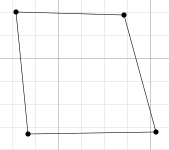
\includegraphics[scale = 0.5]{./figs/simple_graph.png}
        \caption{Simple graph}
    \end{figure}
    We first consider such a simple graph with 4 edges. Without any effort, 
    it has 4 spanning trees, and this result can be applied to a graph with $n$ edges.

    \begin{figure}[h]
        \centering
        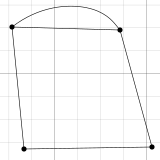
\includegraphics[scale = 0.5]{./figs/simple_multigraph.png}
        \caption{Simple graph}
    \end{figure}
    Then we consider a simple multi-graph case. If we remove one of the parallel edges in the 
    multi-graph, it's exactly a simple graph discussed above. So obviously, we know it has $4 \times 2 = 8$
    spanning trees.

    \begin{figure}[h]
        \centering   
        \subfloat[left part]
        {
            \begin{minipage}[t]{0.5\textwidth}
                \centering     
                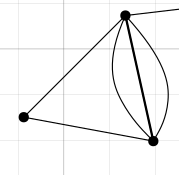
\includegraphics[width=0.5\textwidth]{figs/left-part.png}
            \end{minipage}
        }
        \subfloat[right part]
        {
            \begin{minipage}[t]{0.5\textwidth}
                \centering 
                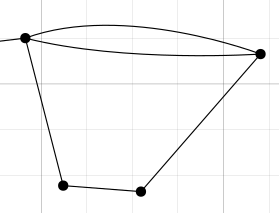
\includegraphics[width=0.5\textwidth]{figs/right-part.png}
            \end{minipage}
        }
    \end{figure}
    Based on these observations, we consider the subgraphs in $Exer.4$. Left part has 3 parallel edges,
    which leads to $3 \times 3 = 9$ spanning trees, and right part has $2 \times 4 = 8$ spanning trees.
    Due to the simple counting method, there're $9 \times 8 = 72$ spanning trees for the graph.Below is some of 
    them.
    \begin{figure}[h]
        \centering
        \subfloat[left part examples]
        {
            \begin{minipage}[t]{0.5\textwidth}
                \centering     
                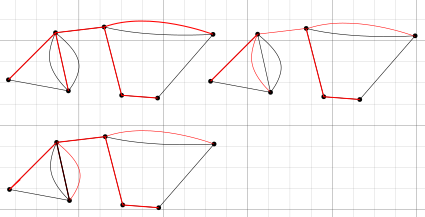
\includegraphics[width=1.0\textwidth]{figs/left-side.png}
            \end{minipage}
        }
        \subfloat[right part examples]
        {
            \begin{minipage}[t]{0.5\textwidth}
                \centering 
                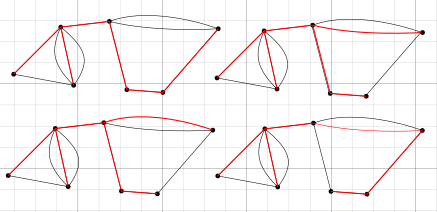
\includegraphics[width=1.0\textwidth]{figs/right-side.png}
            \end{minipage}
        }
    \end{figure}

\subsection*{Exer.5.}
    
    We already know $Prim's$ and $Kruskal's$ algorithm to construct one of the $MST$s of a graph, and 
    only those edges having the same weight may lead to different spanning trees and we have 
    a magic polynomial-time algorithm for cumputing the number of spanning trees.
    Based on these tools, we just need to find do some midifications for $Kruskal's$ algorithm.

    We know that during the process of $Kruskal's$ algorithm, it gets the edges with different weights
    of an $MST$. Having these weights, we can get all other $candidate$ edges for another $MST$ as long 
    as its weight is the same as one of the known $MST$'s edge's. After that, we construct a subgraph $g$
    of graph $G$, and each spanning tree of $g$ is a $MST$ of $G$. Call the magic algorithm, we get the number
    of spanning tree of $g$, which is also the number of $MST$s of $G$. The pseudocode is shown below.

    \begin{algorithm}[H]
        \KwData{graph $G$}
        \KwResult{number of $MST$s of $G$}
        $T$ = Kruskal($G$)\;
        $toMergeEdges$ = $ \emptyset$ \; 
        \For{$e \in T(E)$} {
            \For {$e_{tmp} \in G(E)$} {
                \If {$e.weight == e_{tmp}.weight$ {\bf and} $e \neq e_{tmp}$} {
                    $toMergeEdges = toMergeEdges \cup e_{tmp}$\;
                }
            }
        }
        $T(E) = T(E) \cup toMergeEdges $\;
        $result = $ ComputeSpanningTreeNumber($T$)\;
        \KwRet{$result$}
        \caption{Compute number of $MST$}
       \end{algorithm}

\end{document}

